\documentclass[conference]{IEEEtran}
\usepackage{times}

% numbers option provides compact numerical references in the text.
\usepackage[numbers]{natbib}
\usepackage{multicol}
\usepackage[bookmarks=true]{hyperref}
\usepackage{graphicx}
\usepackage{booktabs}
\usepackage{amsmath}
\usepackage{amssymb}

\pdfinfo{
   /Author (Kewei Liu, Zihao Long, Zihang Zhou)
   /Title  (Temporal Costmap Aggregation for Object-Relative Visual Navigation)
   /Subject (Robot Learning)
   /Keywords (Visual Navigation; Temporal Aggregation; Distribution Shift; Imitation Learning)
}

\begin{document}

\title{Temporal Costmap Aggregation: Mitigating \\ Distribution Shift in Object-Relative Visual Navigation}

\author{Kewei Liu  \quad Zihang Zhou \quad Zihao Long}

\maketitle

\begin{abstract}
ObjectReact~\cite{garg2025objectreact} conditions a local navigation controller on a per-frame ``WayObject Costmap'' rather than raw RGB. A single corrupted costmap can therefore drive the feed-forward policy away from the expert distribution with no temporal signal for recovery. The original single-frame controller reaches $64.4$ clean Avg SPL, while a parameter-free temporal EMA reaches $66.6$. We further compare a plain GRU, a cosine-gated GRU, and a learned reliability-gated GRU in a complete $2{\times}2$ design: training corruption probability $0.0$ or $0.2$, crossed with inference corruption probability $0.0$ or $0.2$. Without training corruption, clean Avg SPL ranges from $36.6$ to $67.3$ and all methods degrade under inference corruption. With training corruption, clean performance narrows to $60.6$--$61.4$ SPL, and the reliability-gated GRU retains $60.2$ SPL under inference corruption, losing only $0.46$ points. However, a step-level mechanism analysis shows that its scalar gate does \emph{not} detect injected failures as intended: using $1-\alpha_t$ as the corruption score gives pooled ROC-AUC $0.312$. The navigation gain therefore cannot be attributed to a calibrated low-reliability detector and should instead be treated as a behavioral property of the jointly trained recurrent architecture. Four automatically selected matched rollouts illustrate this recovery pattern: the reliability model succeeds where plain GRU times out on every task. Results use one training seed, so margins are reported as trends rather than statistically established improvements.
\end{abstract}

\IEEEpeerreviewmaketitle

\section{Problem Statement and Motivation}

Visual navigation in indoor environments is a long-standing problem in embodied AI. Classical geometric methods rely on metric maps and specialized sensors, whereas recent learning-based methods navigate directly from images. ObjectReact~\cite{garg2025objectreact} occupies a promising middle ground: it builds a topometric, object-level scene graph as a prior and trains a local controller on a high-level \emph{WayObject Costmap}, a multi-channel image in which each pixel encodes the planned path length to the goal through the object it belongs to. By conditioning on object-level costs instead of an RGB subgoal image, ObjectReact decouples control from image matching and generalizes well across robot embodiments and trajectories.

The ObjectReact controller, however, is a feed-forward network that consumes \emph{only the current} costmap. Its training data are generated by a shortest-path expert in simulation, and the policy is fit by behavior cloning. It therefore inherits the well-known failure mode of imitation learning: \emph{distribution shift}~\cite{ross2011dagger}. At inference the costmap is recomputed every frame from instantaneous segmentation and matching; when the perception pipeline mismatches segments or misses the goal, the current-frame costmap can become uninformative or misleading, and a single bad frame drives the policy toward a wrong waypoint. Critically, the ObjectReact authors themselves report this limitation: the controller uses no history context, so costmaps that vary sharply frame-to-frame destabilize the prediction, and the agent cannot recover because recovery behavior is absent from the expert demonstrations~\cite{garg2025objectreact}.

Our observation is that although any \emph{single} costmap may be corrupted, a short window of consecutive costmaps usually carries redundant spatial cues and a smooth temporal trend---a driver who loses sight of a sign for one frame relies on the recent past rather than swerving. This motivates our central question: \emph{can a lightweight temporal-memory module recover robustness for ObjectReact without sacrificing its cross-embodiment advantages?} Because naive averaging risks smearing a corrupted frame into the future, we also ask whether a \emph{learned, confidence-gated} aggregator that selectively discounts anomalous frames is needed beyond ungated temporal memory.

This report formulates the temporal-aggregation problem on the WayObject Costmap and evaluates three learned aggregators across the ObjectReact Imitate, Alt-Goal, Shortcut, and Reverse tasks. We evaluate both clean behavior and verified synthetic costmap failures under matched training conditions, allowing us to isolate the value of reliability-aware gating.

\section{Related Work}

\textbf{Object-relative navigation.} RoboHop~\cite{garg2024robohop} introduced segment-based topological maps with a zero-shot controller; TANGO~\cite{podgorski2025tango} added traversability-aware local metric control; ObjectReact~\cite{garg2025objectreact} unified these with a \emph{learned} controller conditioned on a WayObject Costmap, and is the baseline we extend. All operate on single-frame observations. The image-relative line---GNM~\cite{shah2023gnm} and ViNT~\cite{shah2023vint}---predicts control from a current image and a retrieved subgoal image; ObjectReact adapts GNM's pipeline but replaces the goal image with the costmap.

\textbf{Imitation learning and distribution shift.} Behavior cloning compounds errors once the agent leaves the expert distribution~\cite{ross2011dagger}. Remedies include on-policy aggregation (DAgger~\cite{ross2011dagger}) and history-conditioned recurrent policies~\cite{mandlekar2021robomimic}. Our intervention is in the latter family, applied at the costmap-feature level rather than to raw observations.

\textbf{Temporal modeling in navigation.} End-to-end policies commonly stack LSTM/GRU units over a visual encoder~\cite{mirowski2017navigate}; GNM~\cite{shah2023gnm} fuses a short RGB history in its observation encoder, a mechanism ObjectReact dropped for its goal encoder. To our knowledge, no prior work applies a temporal aggregator---let alone a confidence-gated one---to an object-relative costmap representation; this is the gap we target.

\section{Technical Approach}

\begin{figure}[t]
\centering
\includegraphics[width=\columnwidth]{overview.png}
\caption{Overview of our temporal costmap aggregation. We keep the ObjectReact encoder $\phi$ and waypoint head $g$ warm-started from the public checkpoint and trained jointly with the aggregator, and insert an aggregator $\mathcal{A}$ over a sliding window of $K{=}6$ frame embeddings; the confidence-gated variants additionally down-weight frames that disagree with the intra-window history before the GRU integrates them.}
\label{fig:overview}
\end{figure}

\subsection{Background: the ObjectReact controller}
Let $c_t \in \mathbb{R}^{H\times W\times D}$ be the WayObject Costmap at step $t$ ($H{=}64$, $W{=}85$, $D{=}8$ sine--cosine cost channels). ObjectReact applies a custom ResNet goal encoder $\phi$ to obtain a frame embedding $e_t = \phi(c_t) \in \mathbb{R}^{1024}$, and a GNM-style head $g$ predicts a rollout of $T{=}10$ future waypoints $\tau_t = g(e_t)$. We keep the \emph{architecture} of $\phi$ and $g$, the mapping pipeline, the perception pipeline, and the shortest-path expert generator unchanged, warm-starting $\phi$ and $g$ from the public checkpoint and fine-tuning them jointly with the aggregator; our intervention is confined to the step between $\phi$ and $g$ (Fig.~\ref{fig:overview}).

\subsection{Temporal costmap aggregation}
We replace the single embedding $e_t$ with an aggregate $\hat{e}_t$ computed over a sliding window of $K{=}6$ frames, $\{e_{t-K+1},\dots,e_t\}$. The implementation uses \texttt{context\_size}$=5$ and follows the upstream convention $K=\texttt{context\_size}+1$:
\begin{equation}
\tau_t = g\!\left(\hat{e}_t\right), \qquad \hat{e}_t = \mathcal{A}\!\left(e_{t-K+1},\dots,e_t\right).
\end{equation}
We include two non-learned reference systems before comparing three learned
aggregators $\mathcal{A}$. The \emph{original ObjectReact} baseline uses only
the current embedding, $\hat e_t=e_t$. The \emph{Temporal EMA} baseline uses
the same $K{=}6$ window but introduces no trainable temporal parameters:
\begin{equation}
\hat e_t =
\frac{\sum_{j=0}^{K-1}\lambda^{K-1-j}e_{t-K+1+j}}
     {\sum_{j=0}^{K-1}\lambda^{K-1-j}},
\qquad \lambda=0.7.
\end{equation}
These baselines isolate the value of temporal smoothing from learned recurrent
aggregation.

\emph{(1) Plain GRU.} A single-layer GRU (hidden size $1024$) consumes the window and we take its last hidden state, $\hat{e}_t = \mathrm{GRU}(e_{t-K+1},\dots,e_t)$.

\emph{(2) Cosine-confidence--gated GRU.}
Within the window we maintain an intra-window running EMA of past
embeddings,
\begin{equation}
\begin{aligned}
&\bar{e}_{t-K+1} = e_{t-K+1}, \\
&\bar{e}_{j} = \lambda\,\bar{e}_{j-1} + (1-\lambda)\,e_{j} \quad (j = t{-}K{+}2,\dots,t)
\end{aligned}
\end{equation}

with $\lambda{=}0.7$. For each frame $j > t{-}K{+}1$, a scalar
confidence is computed from the cosine similarity between the new
frame and the running mean of the frames that preceded it inside the
window,
\begin{equation}
\alpha_j = \sigma\!\big(w\,\cos(e_j,\,\bar{e}_{j-1}) + b\big),\quad
(w,b)\ \text{learnable},
\end{equation}
and the raw embedding is replaced by a convex blend \emph{before} the
GRU sees it,
\begin{equation}
\tilde{e}_j = \alpha_j\,e_j + (1-\alpha_j)\,\bar{e}_{j-1}.
\end{equation}
The first frame in the window is trusted unconditionally
($\tilde{e}_{t-K+1} = e_{t-K+1}$, $\alpha_{t-K+1}{=}1$).
The GRU then consumes the \emph{gated} sequence and its last hidden
state is the aggregated embedding,
\begin{equation}
\hat{e}_t \;=\; \mathrm{GRU}\!\big(\tilde{e}_{t-K+1},\,\tilde{e}_{t-K+2},\,\dots,\,\tilde{e}_t\big).
\end{equation}
The intuition: rather than letting a corrupted frame perturb the GRU's
hidden state \emph{after} integration, the gate substitutes the
smoothed intra-window history at the \emph{input} level, so the
recurrent integration only ever sees frames it deems consistent with
the local trend. This adds two scalar parameters beyond the plain-GRU.

\emph{(3) Reliability-gated GRU.} The mixing $\tilde{e}_j$ and the GRU
step are identical to (2); only the per-frame confidence $\alpha_j$ is
produced by a learned scorer $s_\psi$ rather than a fixed cosine
statistic. With $d_j = |e_j-\bar{e}_{j-1}|$, $p_j = e_j\odot\bar{e}_{j-1}$,
$c_j = \cos(e_j,\bar{e}_{j-1})$, and
$\delta_j = \|d_j\|_2 / (\|\bar{e}_{j-1}\|_2+\|e_j\|_2+\varepsilon)$,
\begin{equation}
\alpha_j \;=\; \sigma\!\big(\,s_\psi\!\big(\,[\,e_j\,;\,\bar{e}_{j-1}\,;\,d_j\,;\,p_j\,;\,c_j\,;\,\delta_j\,]\,\big)\,\big),
\end{equation}
where $s_\psi$ is a 2-layer MLP (hidden $128$, ReLU). The gate sees
per-channel disagreement signals rather than a single scalar similarity,
at the cost of $\sim$$0.52$M extra parameters.


\subsection{Training}
All learned variants warm-start from the public ObjectReact checkpoint and train end-to-end with the original waypoint-regression loss (MSE over $T{=}10$ waypoints, with $\cos/\sin$ heading channels). We regenerate the data so each sample is a length-$K$ window; the target for a window ending at $t$ is the expert waypoint at $t$. We train two matched sets of all three architectures. One uses $\mathrm{noise\_p}{=}0.0$; the other uses $\mathrm{noise\_p}{=}0.2$, where one random frame embedding is zeroed in an augmented sample. All other settings are shared.

\begin{table}[htbp]
\centering
\caption{Training configuration shared by the learned variants. Each architecture is trained once with noise probability $0.0$ and once with $0.2$.}
\label{tab:train}
\small
\setlength{\tabcolsep}{4pt}
\begin{tabular}{ll}
\toprule
Item & Value \\
\midrule
Initialization & ObjectReact \texttt{object\_react\_latest.pth} \\
Model / context & \texttt{gnm\_temporal}, temporal, $K{=}6$ \\
Goal / obs type & \texttt{image\_mask\_enc} / disabled \\
Epochs / batch & $10$ / $128$ \\
Optimizer / lr & Adam / $7\times10^{-4}$ \\
Seed & $0$ \\
Noise aug. & $\mathrm{noise\_p}\in\{0.0,0.2\}$ (zero one frame) \\
Train split & \texttt{bigger\_bot\_0.3-sh\_0.4} \\
Hardware & single RTX 4090 \\
\bottomrule
\end{tabular}
\end{table}


\section{Experiments and Results}

\subsection{Setup}
We evaluate on the HM3D~\cite{ramakrishnan2021hm3d} InstanceImageNav~\cite{krantz2022iin} validation set (\texttt{hard} difficulty) in Habitat-Sim, using ground-truth topometric goals, over the four ObjectReact tasks: \emph{Imitate} (teach-and-repeat), \emph{Alt-Goal} (reach a seen-but-unvisited goal), \emph{Shortcut} (cut across a longer mapping trajectory), and \emph{Reverse} (traverse the route backward). We report Success Rate (SR), SPL, and Soft-SPL (SSPL). Ground-truth perception isolates the controller from segmentation and matching errors.

All variants are evaluated under a single \textbf{full protocol} (\texttt{evaluate\_objecreact.py}: \texttt{step\_idx}=3, \texttt{end\_idx}=108, \texttt{max\_steps}=300), with blacklist filtering and Alt-Goal included, giving effective episode counts of 33, 23, 26, and 30 for Imitate, Alt-Goal, Shortcut, and Reverse. Goals are provided as ground-truth topometric nodes.

\subsection{Experiment 1: controlled clean evaluation}
\label{sec:clean}

We first report the available original and parameter-free reference
baselines. Both use the public ObjectReact weights without temporal-module
training. Temporal EMA applies the normalized $K{=}6$ embedding average
defined above. They use the same episode range, tasks, blacklist, and metric
script as the learned runs, but were produced with their respective upstream
single-frame and temporal controller configurations. We therefore report them
as contextual baselines rather than as a strict one-variable ablation.

\begin{table}[htbp]
\centering
\caption{Available original and parameter-free clean reference baselines.
Per-task values are SR (\%); the final column reports averaged SR/SPL/SSPL.
The episode and metric protocol is shared, but the historical controller
configurations are not identical.}
\label{tab:nonlearned_baselines}
\small
\setlength{\tabcolsep}{3.5pt}
\begin{tabular}{lcccc c}
\toprule
Method & Imi. & Alt. & Short. & Rev. & Avg SR/SPL/SSPL \\
\midrule
ObjectReact (single frame) & 72.7 & 65.2 & 46.2 & \textbf{73.3} & 64.4 / 64.4 / 75.2 \\
Temporal EMA ($K{=}6$)    & \textbf{75.8} & \textbf{69.6} & \textbf{57.7} & 63.3 & \textbf{66.6} / \textbf{66.6} / \textbf{76.0} \\
\bottomrule
\end{tabular}
\end{table}

Temporal EMA records $2.23$ points higher clean Avg SPL than the original
single-frame run, with higher scores on Imitate, Alt-Goal, and Shortcut but a
$10.0$-point lower Reverse score. Because the historical controller
configurations differ, this gap is descriptive rather than a causal estimate
of EMA's contribution. Temporal EMA nevertheless provides a useful
parameter-free clean reference.

We next evaluate both matched training sets without inference-time
corruption. Within each table, the three architectures share initialization,
training data, seed, temporal window, and training corruption probability.

\begin{table}[htbp]
\centering
\caption{Controlled clean evaluation with
$\mathrm{noise\_p}{=}0.0$ for all three learned variants. Per-task values are
SR (\%); the final column reports averaged SR/SPL/SSPL.}
\label{tab:clean_noise00}
\small
\setlength{\tabcolsep}{3.5pt}
\begin{tabular}{lcccc c}
\toprule
Method & Imi. & Alt. & Short. & Rev. & Avg SR/SPL/SSPL \\
\midrule
Plain GRU             & 75.8 & \textbf{65.2} & \textbf{61.5} & \textbf{66.7} & \textbf{67.3} / \textbf{67.3} / \textbf{75.7} \\
Gated GRU (cosine)    & \textbf{78.8} & 52.2 & 57.7 & 60.0 & 62.2 / 62.2 / 70.8 \\
Reliability-gated GRU & 45.5 & 56.5 & 7.7 & 36.7 & 36.6 / 36.6 / 50.4 \\
\bottomrule
\end{tabular}
\end{table}

Without corruption augmentation, plain GRU is strongest overall and the
reliability-gated model collapses on Shortcut. This is a fair architectural
comparison, but it also shows that the learned reliability mechanism is not
effective without corrupted training examples.

Table~\ref{tab:matched_clean} reports the independently trained
$\mathrm{noise\_p}{=}0.2$ set. Its clean averages are closely matched: the
maximum Avg SPL difference is only $0.78$ points. These values are the
references for the clean-to-noisy deltas in Table~\ref{tab:noise_delta}.

\begin{table}[htbp]
\centering
\caption{Controlled clean evaluation with matched training corruption
($\mathrm{noise\_p}{=}0.2$ for all three learned variants). Per-task values
are SR (\%); the final column reports averaged SR/SPL/SSPL.}
\label{tab:matched_clean}
\small
\setlength{\tabcolsep}{3.5pt}
\begin{tabular}{lcccc c}
\toprule
Method & Imi. & Alt. & Short. & Rev. & Avg SR/SPL/SSPL \\
\midrule
Plain GRU             & \textbf{75.8} & 52.2 & 57.7 & 56.7 & 60.6 / 60.6 / 72.4 \\
Gated GRU (cosine)    & 72.7 & 47.8 & \textbf{61.5} & 63.3 & \textbf{61.4} / \textbf{61.4} / \textbf{72.5} \\
Reliability-gated GRU & 60.6 & \textbf{65.2} & 50.0 & \textbf{66.7} & 60.6 / 60.6 / 72.1 \\
\bottomrule
\end{tabular}
\end{table}

\subsection{Experiment 2: controlled inference-time corruption}
\label{sec:noise}

At each control step, the current WayObject Costmap is independently replaced by a zero map with probability $0.2$ \emph{before} it enters temporal history. A fixed seed and episode identifier generate the same corruption schedule for every method. Logged corruption rates range from $19.41\%$ to $20.20\%$ across all 24 runs.

\begin{table}[htbp]
\centering
\caption{Inference-noise evaluation for models trained with
$\mathrm{noise\_p}{=}0.0$. Per-task values are SR (\%); the final column
reports averaged SR/SPL/SSPL.}
\label{tab:noise_train00}
\small
\setlength{\tabcolsep}{3.5pt}
\begin{tabular}{lcccc c}
\toprule
Method & Imi. & Alt. & Short. & Rev. & Avg SR/SPL/SSPL \\
\midrule
Plain GRU             & \textbf{72.7} & \textbf{56.5} & 50.0 & 53.3 & \textbf{58.1} / \textbf{58.1} / \textbf{69.4} \\
Gated GRU (cosine)    & 66.7 & 39.1 & \textbf{57.7} & \textbf{63.3} & 56.7 / 56.7 / 68.4 \\
Reliability-gated GRU & 30.3 & 47.8 & 0.0 & 20.0 & 24.5 / 24.5 / 39.9 \\
\bottomrule
\end{tabular}
\end{table}

\begin{table}[htbp]
\centering
\caption{Clean-to-noisy change for models trained with
$\mathrm{noise\_p}{=}0.0$. Higher deltas are better.}
\label{tab:noise_delta_train00}
\small
\setlength{\tabcolsep}{5pt}
\begin{tabular}{lrrr}
\toprule
Method & $\Delta$ Avg SR & $\Delta$ Avg SPL & $\Delta$ Avg SSPL \\
\midrule
Plain GRU             & $-9.15$ & $-9.15$ & $-6.29$ \\
Gated GRU (cosine)    & $\mathbf{-5.46}$ & $\mathbf{-5.46}$ & $\mathbf{-2.41}$ \\
Reliability-gated GRU & $-12.05$ & $-12.05$ & $-10.42$ \\
\bottomrule
\end{tabular}
\end{table}

Without training corruption, plain GRU has the best absolute noisy result,
while cosine gating has the smallest degradation. Reliability gating is weak
even on clean evaluation and degrades further under inference corruption.

\begin{table}[htbp]
\centering
\caption{Inference-noise evaluation for models trained with
$\mathrm{noise\_p}{=}0.2$. Per-task values are SR (\%); the final column
reports averaged SR/SPL/SSPL.}
\label{tab:noise}
\small
\setlength{\tabcolsep}{3.5pt}
\begin{tabular}{lcccc c}
\toprule
Method & Imi. & Alt. & Short. & Rev. & Avg SR/SPL/SSPL \\
\midrule
Plain GRU             & \textbf{69.7} & 47.8 & \textbf{57.7} & 60.0 & 58.8 / 58.8 / 69.4 \\
Gated GRU (cosine)    & 66.7 & 39.1 & 53.9 & 60.0 & 54.9 / 54.9 / 68.7 \\
Reliability-gated GRU & 63.6 & \textbf{60.9} & 46.2 & \textbf{70.0} & \textbf{60.2} / \textbf{60.2} / \textbf{74.0} \\
\bottomrule
\end{tabular}
\end{table}

\begin{table}[htbp]
\centering
\caption{Robustness relative to each model's matched-training-noise clean evaluation. Higher deltas are better.}
\label{tab:noise_delta}
\small
\setlength{\tabcolsep}{5pt}
\begin{tabular}{lrrr}
\toprule
Method & $\Delta$ Avg SR & $\Delta$ Avg SPL & $\Delta$ Avg SSPL \\
\midrule
Plain GRU             & $-1.77$ & $-1.77$ & $-3.03$ \\
Gated GRU (cosine)    & $-6.45$ & $-6.44$ & $-3.76$ \\
Reliability-gated GRU & $\mathbf{-0.46}$ & $\mathbf{-0.46}$ & $\mathbf{+1.93}$ \\
\bottomrule
\end{tabular}
\end{table}

\textbf{Reliability gating becomes robust after corruption augmentation.} It reaches $60.2$ Avg SPL under corruption, $1.36$ points above the matched plain GRU and $5.25$ above the matched cosine-gated GRU. It also retains its clean Avg SPL within $0.46$ points. The gains concentrate on Alt-Goal and Reverse, whereas plain GRU remains strongest on Imitate and Shortcut.

\textbf{Architecture and augmentation interact strongly.} Cosine gating loses $6.44$ Avg SPL from clean to noisy evaluation, whereas the reliability-gated architecture loses only $0.46$. This establishes a behavioral difference between the two architectures, but does not by itself establish that the reliability score is a calibrated failure detector. We test that mechanism directly in Sec.~\ref{sec:gate_analysis}.

\subsection{Complete $2{\times}2$ comparison}
\label{sec:two_by_two}

Table~\ref{tab:two_by_two} condenses the complete controlled design into one
fair comparison. Every cell uses the same evaluation protocol and differs only
in training and inference corruption probability. The table exposes the key
interaction: reliability gating is the weakest method when trained without
corruption, but becomes the strongest under inference corruption after
matched augmentation. Plain GRU changes little across training conditions,
whereas cosine gating does not benefit from corruption training.

\begin{table*}[t]
\centering
\caption{Complete $2{\times}2$ training-noise by inference-noise comparison.
Values are Avg SPL over Imitate, Alt-Goal, Shortcut, and Reverse. Within each
column, all architectures use the same training corruption, inference
corruption, data, seed, temporal window, and evaluation protocol.}
\label{tab:two_by_two}
\small
\setlength{\tabcolsep}{10pt}
\begin{tabular}{lcc cc}
\toprule
& \multicolumn{2}{c}{Train noise $0.0$}
& \multicolumn{2}{c}{Train noise $0.2$} \\
\cmidrule(lr){2-3}\cmidrule(lr){4-5}
Method & Eval $0.0$ & Eval $0.2$ & Eval $0.0$ & Eval $0.2$ \\
\midrule
Plain GRU             & \textbf{67.30} & \textbf{58.14} & 60.57 & 58.80 \\
Gated GRU (cosine)    & 62.16 & 56.70 & \textbf{61.35} & 54.91 \\
Reliability-gated GRU & 36.56 & 24.52 & 60.62 & \textbf{60.16} \\
\bottomrule
\end{tabular}
\end{table*}

\subsection{Experiment 3: does the gate detect corrupted frames?}
\label{sec:gate_analysis}

The behavioral results motivate a stricter mechanism test. For both
reliability checkpoints (trained with corruption probability $0.0$ and
$0.2$), we repeat all four noisy evaluations while logging the full
$K{=}6$ gate vector and its current-frame value $\alpha_t$ at every control
step. The inference-noise injector independently records whether the current
costmap was zeroed, providing a direct binary failure label. The diagnostic
runs exactly reproduce the original navigation outcomes: success status and
final distance match for all 111 non-blacklisted episodes shared with the
original reliability evaluation.

Because a lower $\alpha_t$ is intended to indicate lower reliability, we use
$1-\alpha_t$ as the corruption-detection score. We report pooled and
per-task ROC-AUC and average precision (AP), with 95\% confidence intervals
from 2,000 episode-cluster bootstrap samples (seed 42). Table~\ref{tab:gate}
shows the pooled result.

\begin{table}[t]
\centering
\caption{Pooled gate-detection results under inference corruption probability
$0.2$. Positive labels are injected zero-costmap frames and the detection
score is $1-\alpha_t$. Confidence intervals use episode-cluster bootstrap.
AP should be compared with the approximately $19.5\%$ positive rate.}
\label{tab:gate}
\small
\setlength{\tabcolsep}{4pt}
\begin{tabular}{lcc cc}
\toprule
Train noise & ROC-AUC & AP & $\bar{\alpha}_{\rm clean}$ & $\bar{\alpha}_{\rm inj.}$ \\
\midrule
$0.0$ & 0.255 {\scriptsize[0.239, 0.271]} &
0.191 {\scriptsize[0.185, 0.196]} & 1.0000 & 1.0000 \\
$0.2$ & 0.312 {\scriptsize[0.285, 0.337]} &
0.136 {\scriptsize[0.130, 0.143]} & 0.9880 & 0.9984 \\
\bottomrule
\end{tabular}
\end{table}

\begin{figure}[t]
\centering
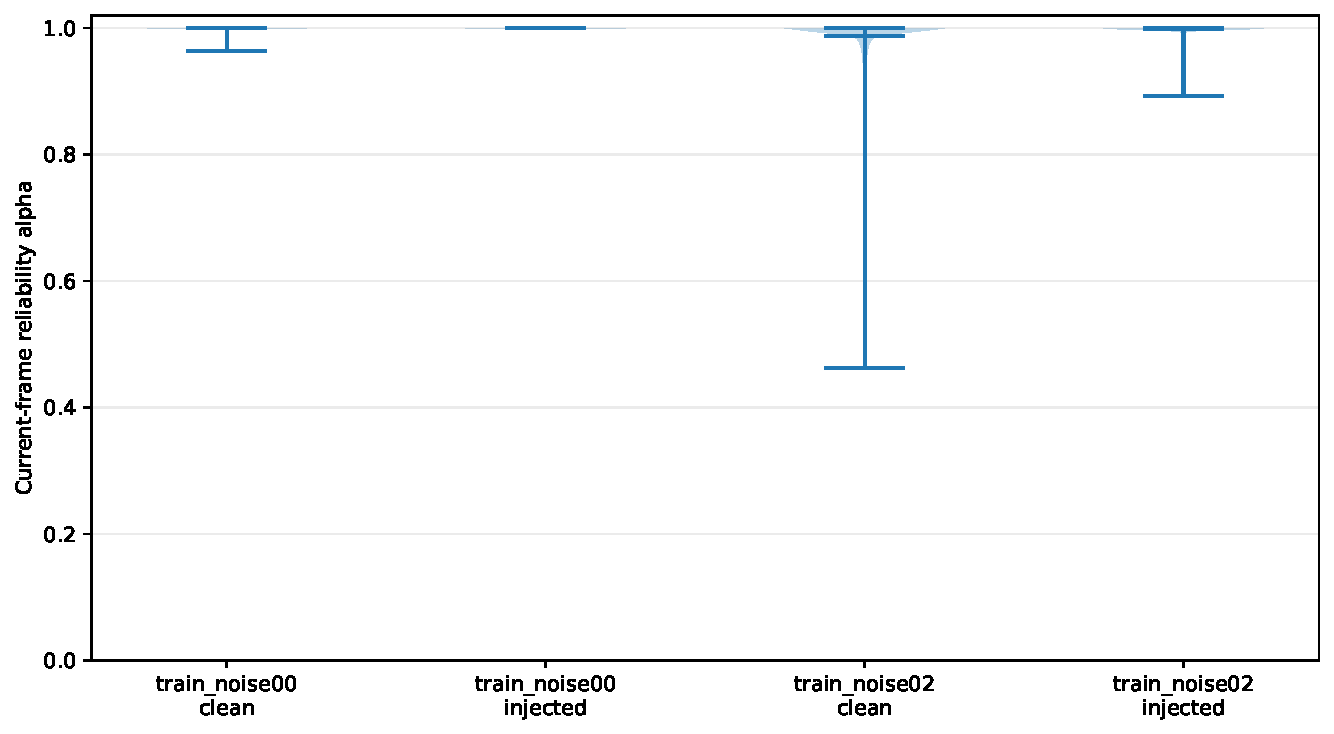
\includegraphics[width=\columnwidth]{paper_figures/gate_alpha_distributions.pdf}
\caption{Current-frame gate values for clean and injected steps. The
noise-free checkpoint saturates near one. After corruption training, clean
steps have greater variance and a \emph{lower} mean alpha than injected
steps---the opposite of the intended reliability semantics.}
\label{fig:alpha_distribution}
\end{figure}

\begin{figure*}[t]
\centering
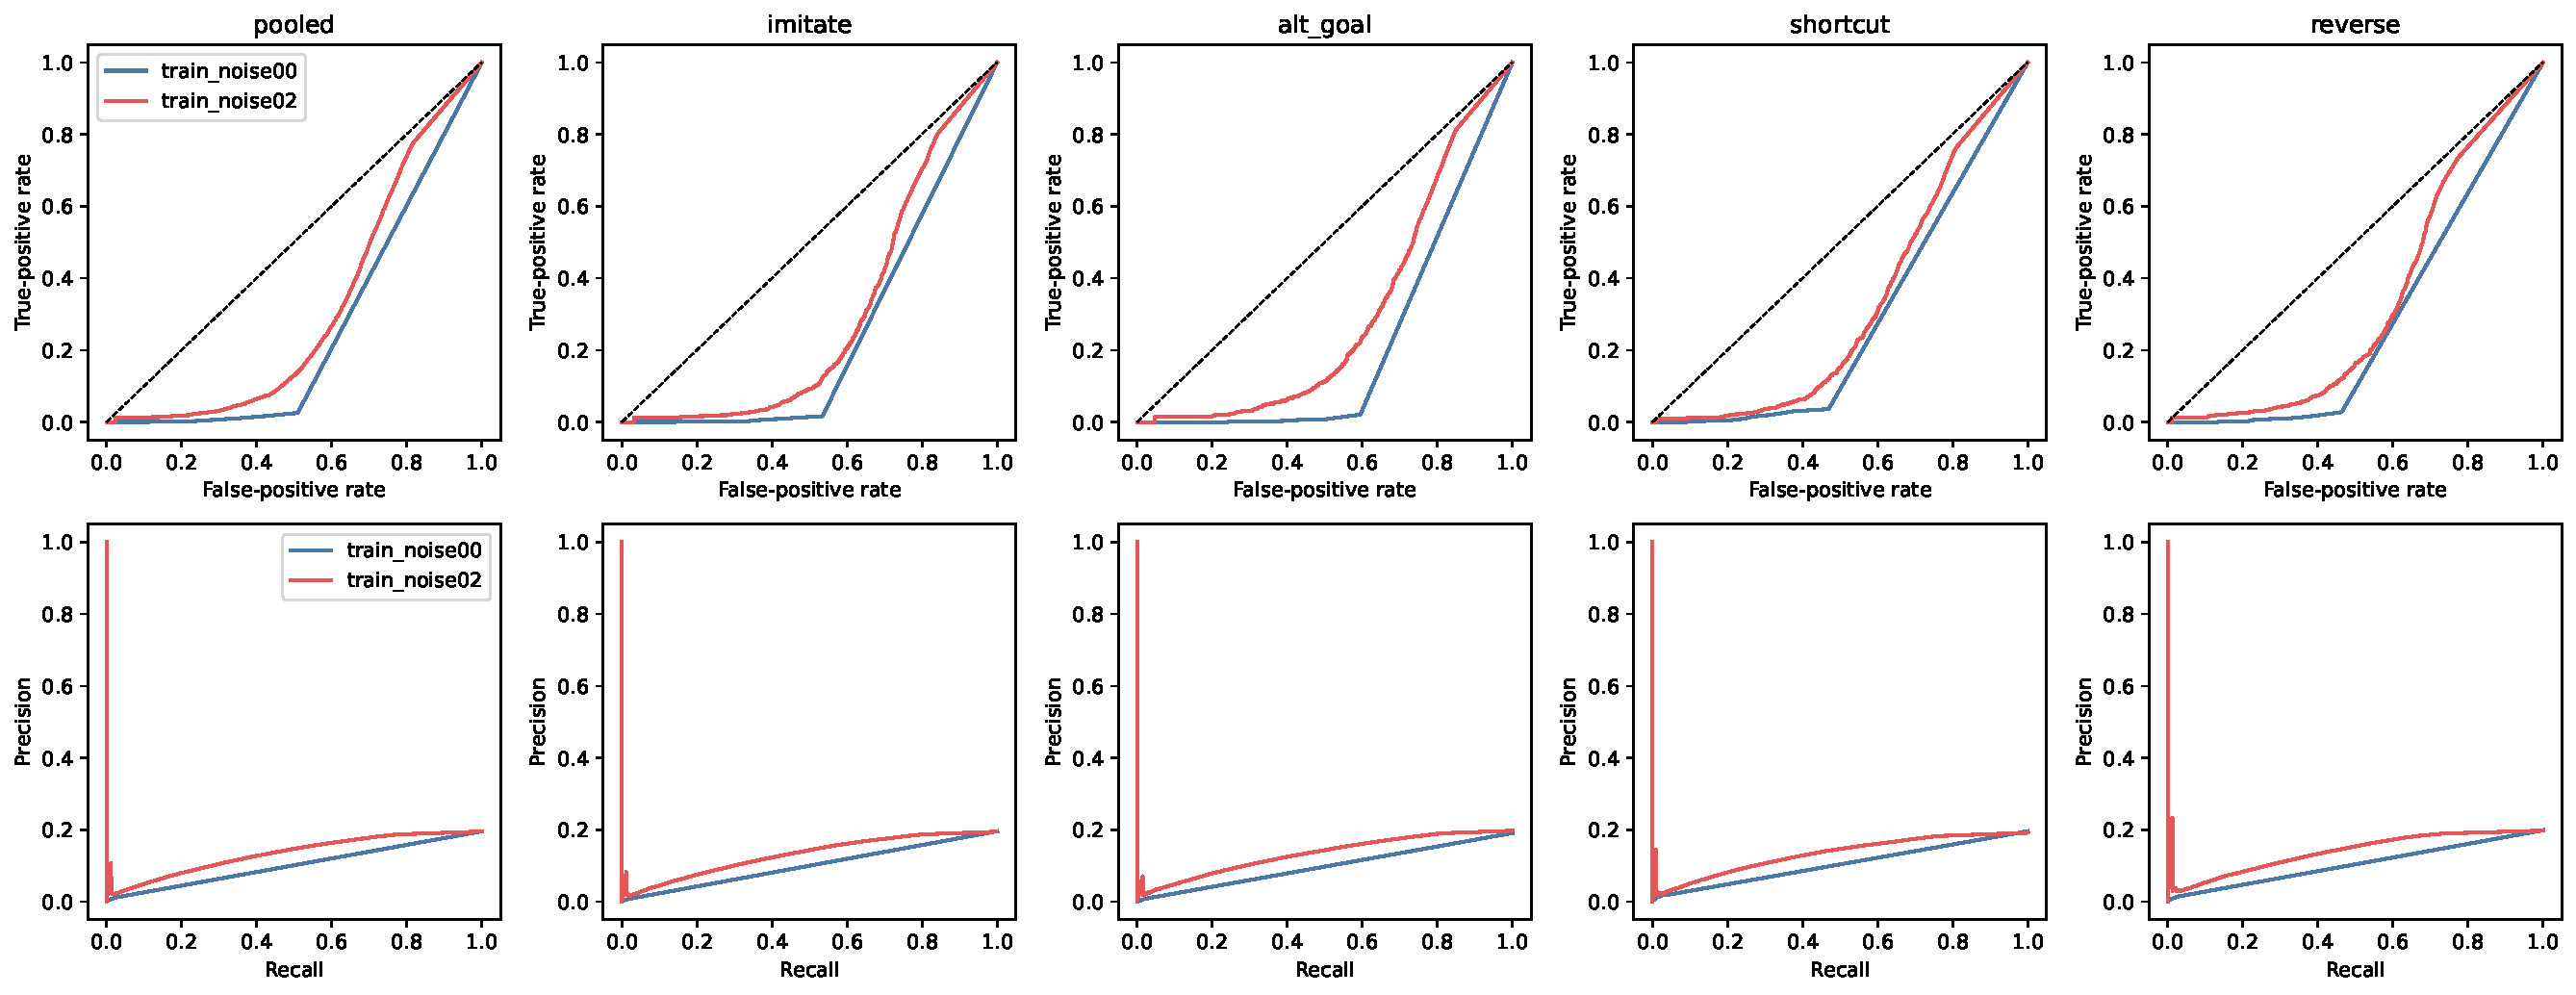
\includegraphics[width=\textwidth]{paper_figures/gate_roc_pr_curves.pdf}
\caption{ROC (top) and precision--recall (bottom) curves for pooled and
per-task corruption detection. All ROC curves lie below the chance diagonal
when $1-\alpha_t$ is used as the detector. The failure is consistent across
all four tasks rather than being caused by one task.}
\label{fig:gate_curves}
\end{figure*}

\textbf{The learned score does not behave as a reliability detector.}
Both pooled ROC-AUC values are below $0.5$, and every per-task ROC-AUC is
between $0.209$ and $0.333$. The unaugmented gate is almost fully saturated at
one. Corruption training increases score variation, but in the wrong
direction: injected frames receive mean alpha $0.9984$, compared with
$0.9880$ on clean frames (Fig.~\ref{fig:alpha_distribution}). Its AP of
$0.136$ is also below the injected-frame prevalence. Consequently, the
navigation improvement in Table~\ref{tab:two_by_two} cannot be attributed to
the scorer explicitly identifying and suppressing zero-costmap frames.
A more defensible interpretation is that task-loss training changes the
combined gate--GRU dynamics and recurrent representation, while leaving the
scalar gate uncalibrated. Explicit corruption supervision or a calibration
loss is needed before $\alpha_t$ can be interpreted as reliability.

\subsection{Experiment 4: matched qualitative rollouts}
\label{sec:qualitative}

We next compare the corruption-trained Plain GRU and Reliability-Gated GRU
under the same inference-noise probability $0.2$. For each task, we
automatically select a non-blacklisted episode where reliability gating
succeeds and Plain GRU fails, prioritizing the largest reduction in final
goal distance. This produces one strict matched pair per task; no episode is
chosen from different start states or corruption schedules.

\begin{table}[t]
\centering
\caption{Matched qualitative cases. Plain GRU reaches the 300-step limit in
all four episodes, while Reliability-Gated GRU succeeds. Distances are meters
from the goal at termination.}
\label{tab:qualitative}
\small
\setlength{\tabcolsep}{3.5pt}
\begin{tabular}{lrrr}
\toprule
Task & Plain dist. & Reliability dist. & Improvement \\
\midrule
Imitate  & 2.729 & 0.993 & 1.735 \\
Alt-Goal & 6.875 & 0.978 & 5.897 \\
Shortcut & 8.710 & 0.991 & 7.719 \\
Reverse  & 5.741 & 0.996 & 4.746 \\
\bottomrule
\end{tabular}
\end{table}

\begin{figure*}[t]
\centering
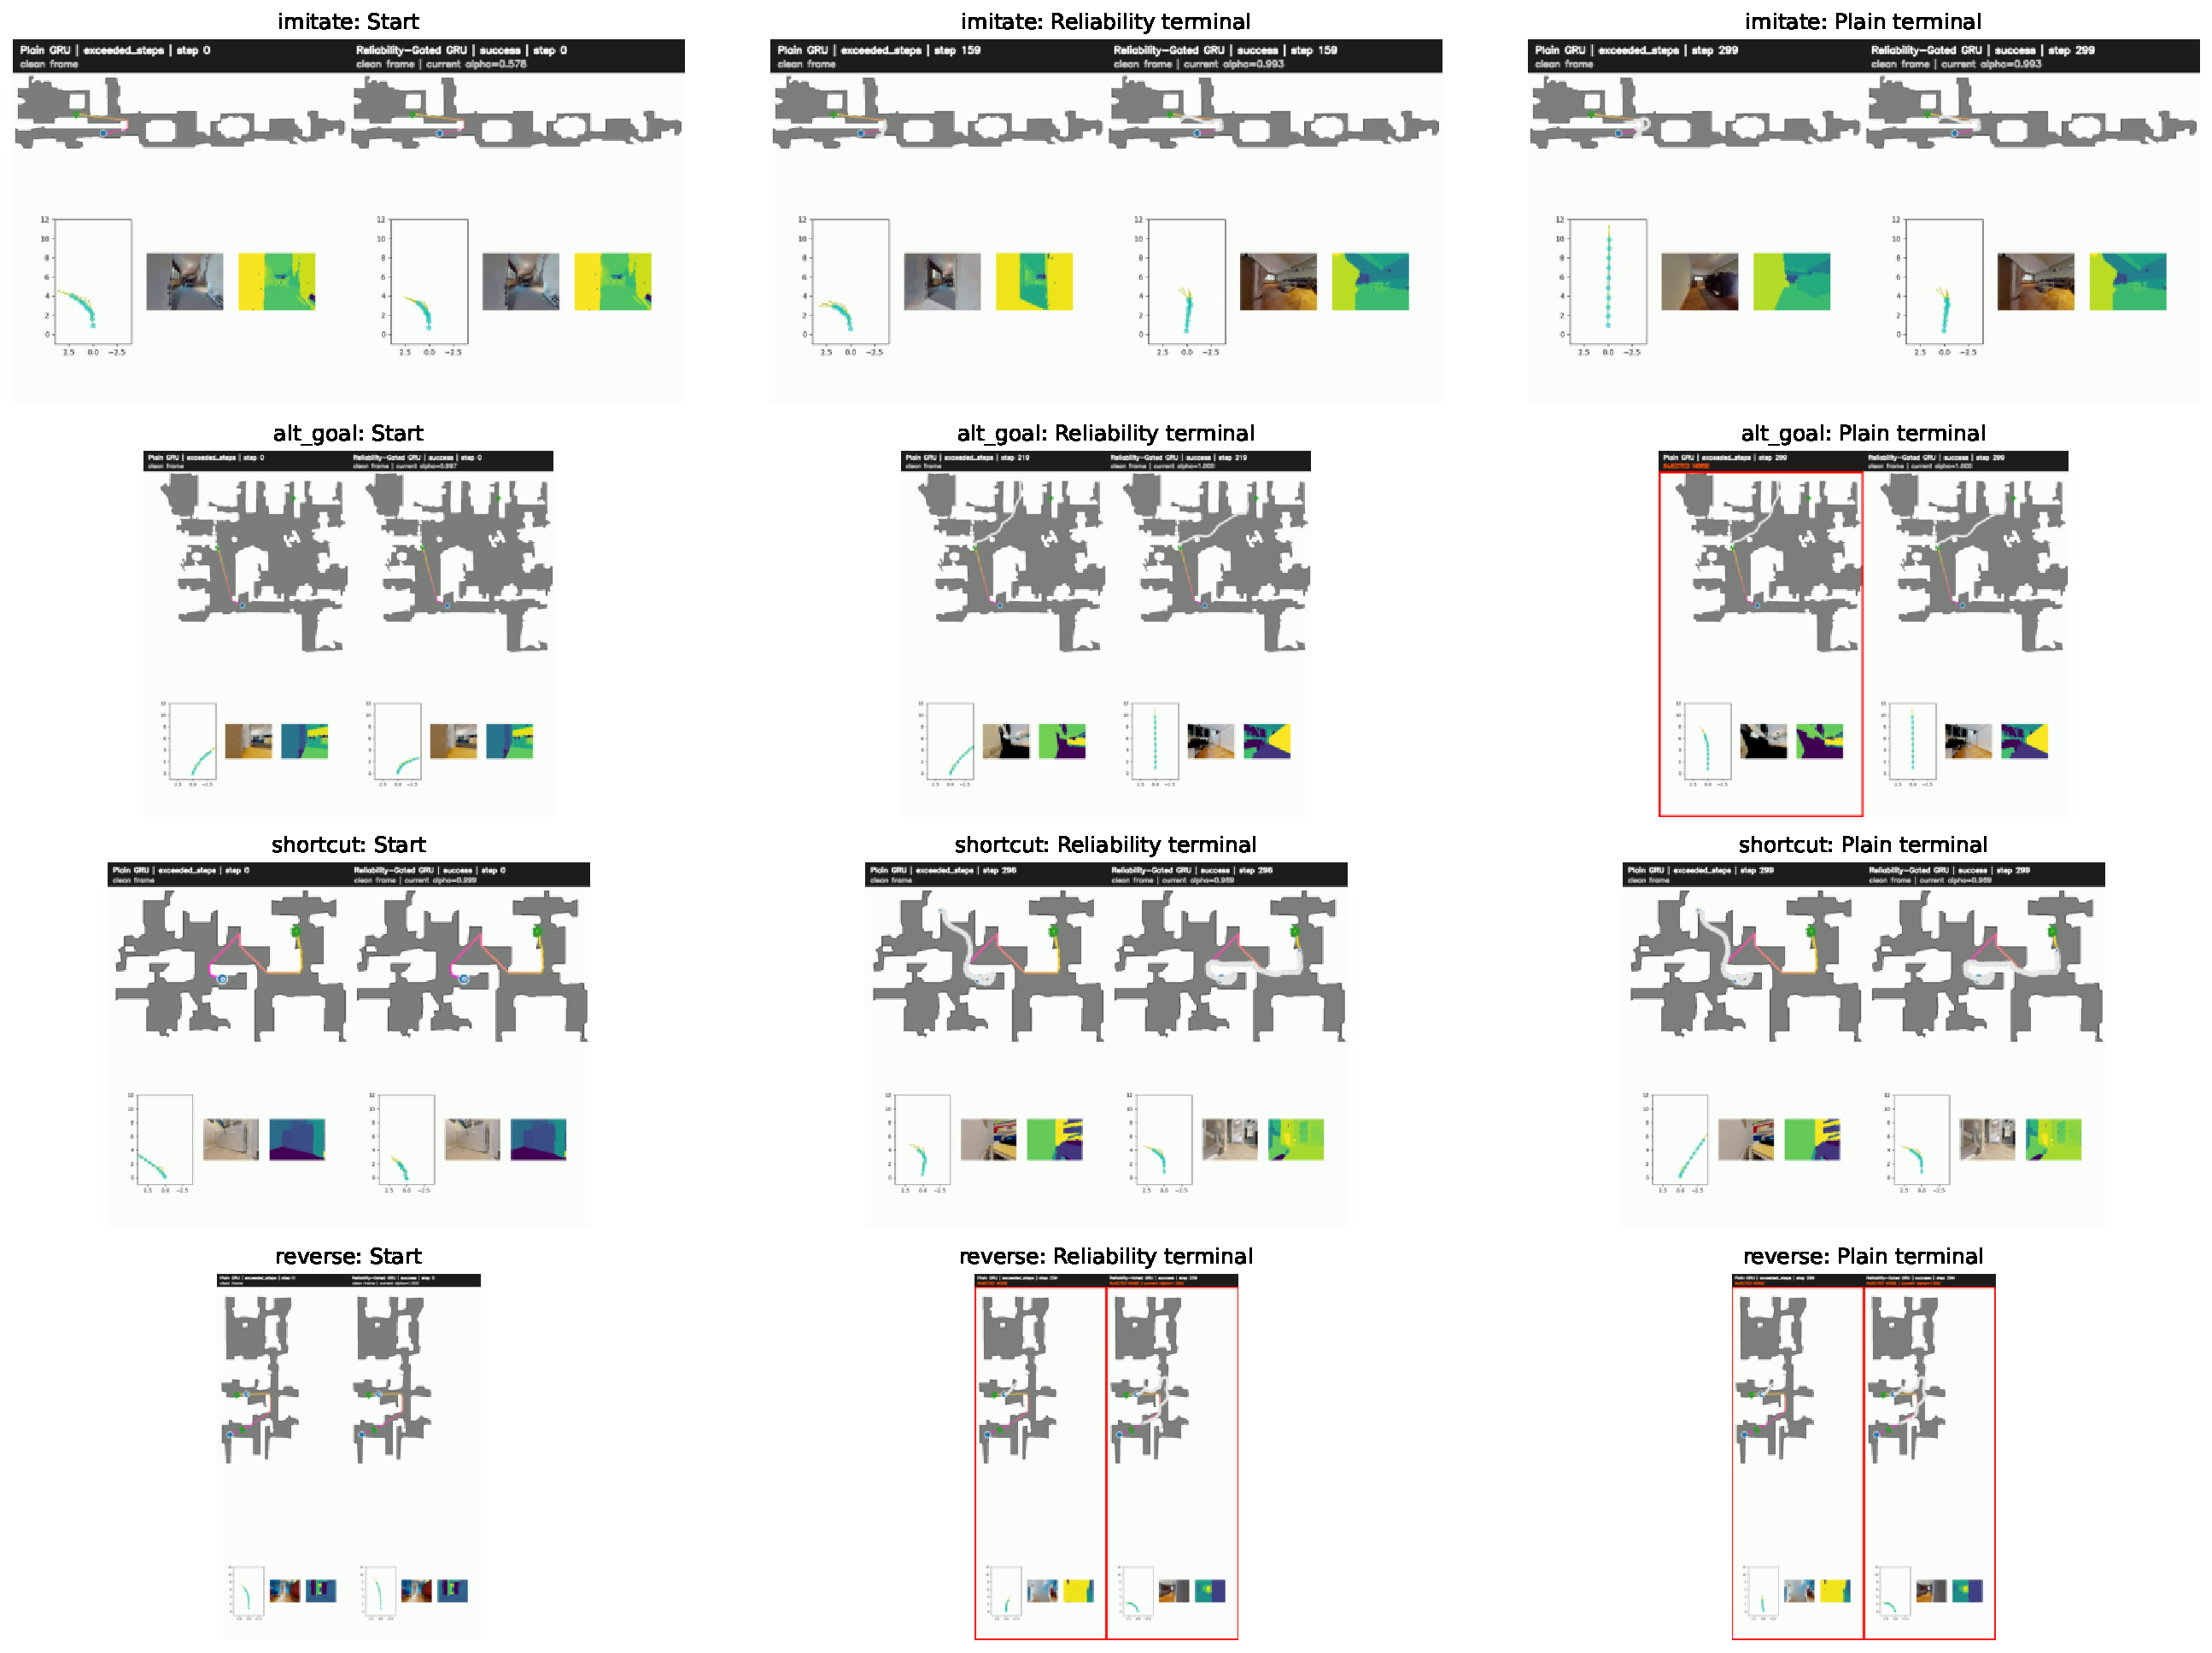
\includegraphics[width=\textwidth]{paper_figures/matched_rollouts_contact_sheet.pdf}
\caption{Matched rollout contact sheet. Rows are Imitate, Alt-Goal, Shortcut,
and Reverse; columns show the common start, the time when the reliability
model terminates successfully, and the Plain-GRU terminal time. Each cell
contains synchronized Plain-GRU (left) and Reliability-Gated-GRU (right)
views. Red borders mark injected-noise steps. The full 6\,fps side-by-side
rollouts are provided as supplementary MP4 files.}
\label{fig:qualitative}
\end{figure*}

Figure~\ref{fig:qualitative} shows that the difference is not a small
threshold effect. On Alt-Goal, Shortcut, and Reverse, Plain GRU remains several
meters from the goal after 300 steps, while the reliability model reaches
within one meter. On Imitate, Plain GRU approaches the goal but fails to
complete, whereas the reliability model succeeds at step 159. These examples
support the aggregate robustness result behaviorally, but they do not rescue
the detector interpretation rejected by Sec.~\ref{sec:gate_analysis}: the
model can recover under corruption even though its scalar alpha is not a
calibrated failure score.

\subsection{Summary of findings}
The results separate clean performance from corruption robustness.

\emph{Clean behavior.} Under matched $\mathrm{noise\_p}{=}0.0$ training, plain GRU is strongest and reliability gating performs poorly. Under matched $\mathrm{noise\_p}{=}0.2$ training, the three methods have nearly tied clean averages ($60.6$--$61.4$ SPL). Training corruption therefore has a large architecture-dependent effect and is essential for the learned reliability gate.

\emph{Robustness.} Training corruption interacts strongly with architecture.
For reliability gating, it raises noisy Avg SPL from $24.5$ to $60.2$ and
changes the clean-to-noisy loss from $12.05$ to $0.46$ points. Plain GRU gains
only $0.66$ noisy SPL from training corruption, while cosine gating loses
$1.79$. The benefit is therefore specific to the jointly trained
reliability-gated recurrent architecture, not a generic effect of
augmentation. However, the gate diagnostic shows that this benefit is not
implemented as the intended low-alpha corruption detector.

\section{Limitations}
\label{sec:limitations}
We state the scope of these claims explicitly.

\begin{itemize}
\item \textbf{Synthetic corruption.} The robustness experiment uses zero-map failures under ground-truth perception. This is controlled and auditable, but it does not reproduce the full structure of FastSAM/LightGlue errors.
\item \textbf{Baseline corruption coverage.} Original ObjectReact and
Temporal EMA have verified clean evaluations, but their earlier
\texttt{noise}/\texttt{EMA+noise} runs predate the corrected inference
injector and are therefore excluded. The noisy $2{\times}2$ comparison is
restricted to the three learned GRU variants.
\item \textbf{Historical baseline configuration.} The reported ObjectReact
and Temporal EMA clean references share the episode and metric protocol, but
come from their respective upstream and temporal controller configurations.
They are included for context and are not used as a strict architectural
ablation.
\item \textbf{Modest episode budget.} Each task has at most 36 raw episodes and fewer after blacklist filtering. The $1.36$ Avg SPL margin between reliability-gated and plain GRU should be treated as a trend.
\item \textbf{Single seed.} All learned variants use training seed 0; seed variance has not been measured.
\item \textbf{Dataset failures.} Shortcut contains two known missing-data episodes and one non-blacklisted episode without a success status. All methods are evaluated with the same handling.
\item \textbf{Uncalibrated gate semantics.} The reliability architecture is robust behaviorally, but its scalar alpha is saturated and anti-correlated with injected failures under the intended interpretation. It should not be presented as an interpretable reliability probability.
\item \textbf{Qualitative selection.} The matched videos deliberately select episodes where the methods differ and therefore illustrate failure modes rather than estimate their population frequency; aggregate rates are reported separately.
\end{itemize}



\section{Remaining Work}
\label{sec:plan}
\begin{enumerate}
\item \textbf{Inferred-perception evaluation.} Replace ground-truth segmentation with FastSAM~\cite{zhao2023fastsam} and LightGlue~\cite{lindenberger2023lightglue} to test naturally structured perception failures.
\item \textbf{Multiple seeds and corruption levels.} Repeat training and evaluate a sweep over inference-noise probabilities to quantify variance and robustness curves.
\item \textbf{Explicit gate supervision.} Add a corruption-classification or calibration objective so that low alpha has an identifiable reliability meaning, then repeat the detection analysis on synthetic and natural failures.
\end{enumerate}

\section{Conclusion}
\label{sec:conclusion}
We targeted ObjectReact's single-frame brittleness with lightweight temporal aggregation and completed a fair $2{\times}2$ training-noise by inference-noise study. The results show a strong architecture--augmentation interaction. Reliability gating fails without corrupted training examples but, after training with $\mathrm{noise\_p}{=}0.2$, becomes the strongest and most stable model under inference corruption, reaching $60.2$ Avg SPL with only a $0.46$-point loss. Four matched rollouts confirm recovery cases across all tasks. Mechanism analysis, however, rejects the simplest explanation for this gain: the learned alpha does not identify injected failures and is not an interpretable reliability probability. The strongest supported conclusion is therefore behavioral---corruption-trained reliability-gated recurrence is robust---while explicit supervision is needed to make the gate itself reliable and explainable.

\section*{Acknowledgments}
We build on the public ObjectReact codebase and the Habitat/HM3D ecosystem. Our repository is at \url{https://github.com/6chHenry/object-rel-nav}.

{\footnotesize
\setlength{\bibsep}{2pt plus 0.4ex}
\bibliographystyle{plainnat}
\bibliography{references}
}

\end{document}
